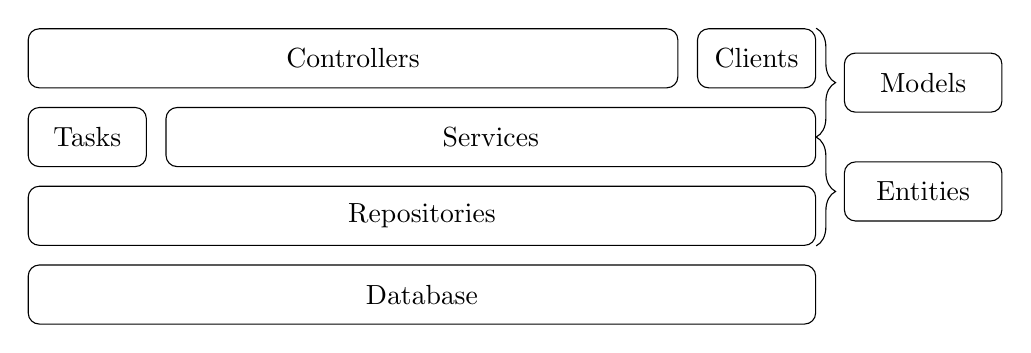
\begin{tikzpicture}%\tikzstyle{every node}=[font=\small]
\node[draw, rounded corners, minimum width = 10cm, minimum height = 0.75cm, anchor=west] (db) at (0,0) {Database};
\node[draw, rounded corners, minimum width = 10cm, anchor=west, minimum height = 0.75cm] (repo) at (0,1) {Repositories};
\node[draw, rounded corners, minimum width = 1.5cm, anchor=west, minimum height = 0.75cm] (tasks) at (0,2) {Tasks};
\node[draw, rounded corners, minimum width = 8.25cm, anchor=west, minimum height = 0.75cm] (services) at (1.75,2) {Services};
\node[draw, rounded corners, minimum width = 8.25cm, anchor=west, minimum height = 0.75cm] (controllers) at (0,3) {Controllers};
\node[draw, rounded corners, minimum width = 1.5cm, anchor=west, minimum height = 0.75cm] (clients) at (8.5,3) {Clients};
%%%%%%%%%%%
\draw [decorate,decoration={brace,amplitude=7pt}] (clients.north east) -- node[draw, rounded corners, minimum width = 2cm, anchor=west, minimum height = 0.75cm, midway, xshift=10pt] {Models} (services.east);
\draw [decorate,decoration={brace,amplitude=7pt}] (services.east) -- node[draw, rounded corners, minimum width = 2cm, anchor=west, minimum height = 0.75cm, midway, xshift=10pt] {Entities} (repo.south east);
\end{tikzpicture}